\documentclass[UTF8,twocolum,titlepage]{ctexart}
\usepackage{graphicx}
\usepackage{placeins}
\usepackage{float}
\usepackage{enumerate}
\usepackage{geometry}
\usepackage{amsmath,bm}
\usepackage{url}
% \setCJKfamilyfont{deffont}{simkai.ttf}
\geometry{left=3cm,right=3cm,top=2.5cm,bottom=2.5cm}
\title{自然对数的数值计算}
\author{孙大伟 2014010782}
\date{}

\begin{document}
\maketitle
\boldmath
\section*{需求分析}
\paragraph{}
使用数值方法计算$ln\left(x\right)$,要求精度高于$10^{-20}$。
\section*{方案设计}
\paragraph{}
输入$x$,然后选取一种计算方法进行计算。计算方法包括泰勒级数法,数值积分法,反双曲正切法。由于编程语言内建的浮点数类型不足以支持作业要求的精度,所以需要实现任意精度的四则运算。
\paragraph{}
因为输入的$x$范围较大,不便于控制误差,所以在每种方法计算之前都作变换$$t=\frac{x}{e^{ceil\left(ln\left(x\right)\right)}}$$ $$ln\left(x\right)=ln\left(t\right)+e*ceil\left(ln\left(x\right)\right)$$其中$ceil\left(f\right)$表示对$f$上取整,此变换将操作数变换到区间$\left(\frac{1}{e},1 \right]$上。以下对每种方法的介绍都是假设操作数在区间$\left(\frac{1}{e},1 \right]$上。由于$e$的值可以通过其他途径得到,且除法的误差不做考虑,所以此变换的误差可忽略。
\subsection*{泰勒级数法}
对$ln\left(t\right)$做泰勒展开,因为$t\in\left(\frac{1}{e},1 \right]$,所以泰勒级数收敛到$ln\left(t\right)$。
$$ln\left(t\right)=\sum\limits_{n=1}^{\infty}\frac{\left(-1\right)^{n-1}*\left(t-1\right)^{n}}{n}$$
\subsection*{数值积分法}
\paragraph{}
因为$$ln\left(t\right)=\int_1^t \frac{1}{x}\,dx$$所以可以使用数值积分方法得到$ln\left(t\right)$的值。实验中使用了龙贝格算法进行计算,即
\begin{eqnarray*}
R_n&=&\frac{64}{63}C_{2n}-\frac{1}{63}C_{n}\\
&=&\frac{64*16}{63*65}S_{4n}-\frac{64+16}{63*65}S_{2n}+\frac{1}{63*65}S_{n}
\end{eqnarray*}
其中
$$S_n=\frac{h}{6}\left[f(a)+f(b)+2\sum_{k=1}^{n-1}f(x_{k})+4\sum_{k=0}^{n-1}f(x_{k}+\frac{h}{2})\right]$$
\paragraph{积分方法的确定}
复化积分法外推加速公式\\
$$T_m^{(k)}=\frac{4^m}{4^m-1}T_{m-1}^{k+1}-\frac{1}{4^m-1}T_{m-1}^{k}$$
加速一次收敛速度提升2阶,需要计算的项数变为3倍。$T_m^{(k)}$的收敛速度为$\left(\frac{L}{2^k}\right)^{2m+2}$,需要计算$N=3^m\cdot2^k$项。固定收敛速度为$\varepsilon=10^{-20}$,则有$$\left(\frac{L}{2^k}\right)^{2m+2}=\varepsilon$$ $$N=3^m\cdot\frac{L}{\varepsilon^{\frac{1}{2m+2}}}$$所以得到加速次数与计算项数的关系如图\ref{fig:integration_m},从图中可以看出,选择$m=3$比较合理,即龙贝格公式。
\begin{figure}[H]
\centering
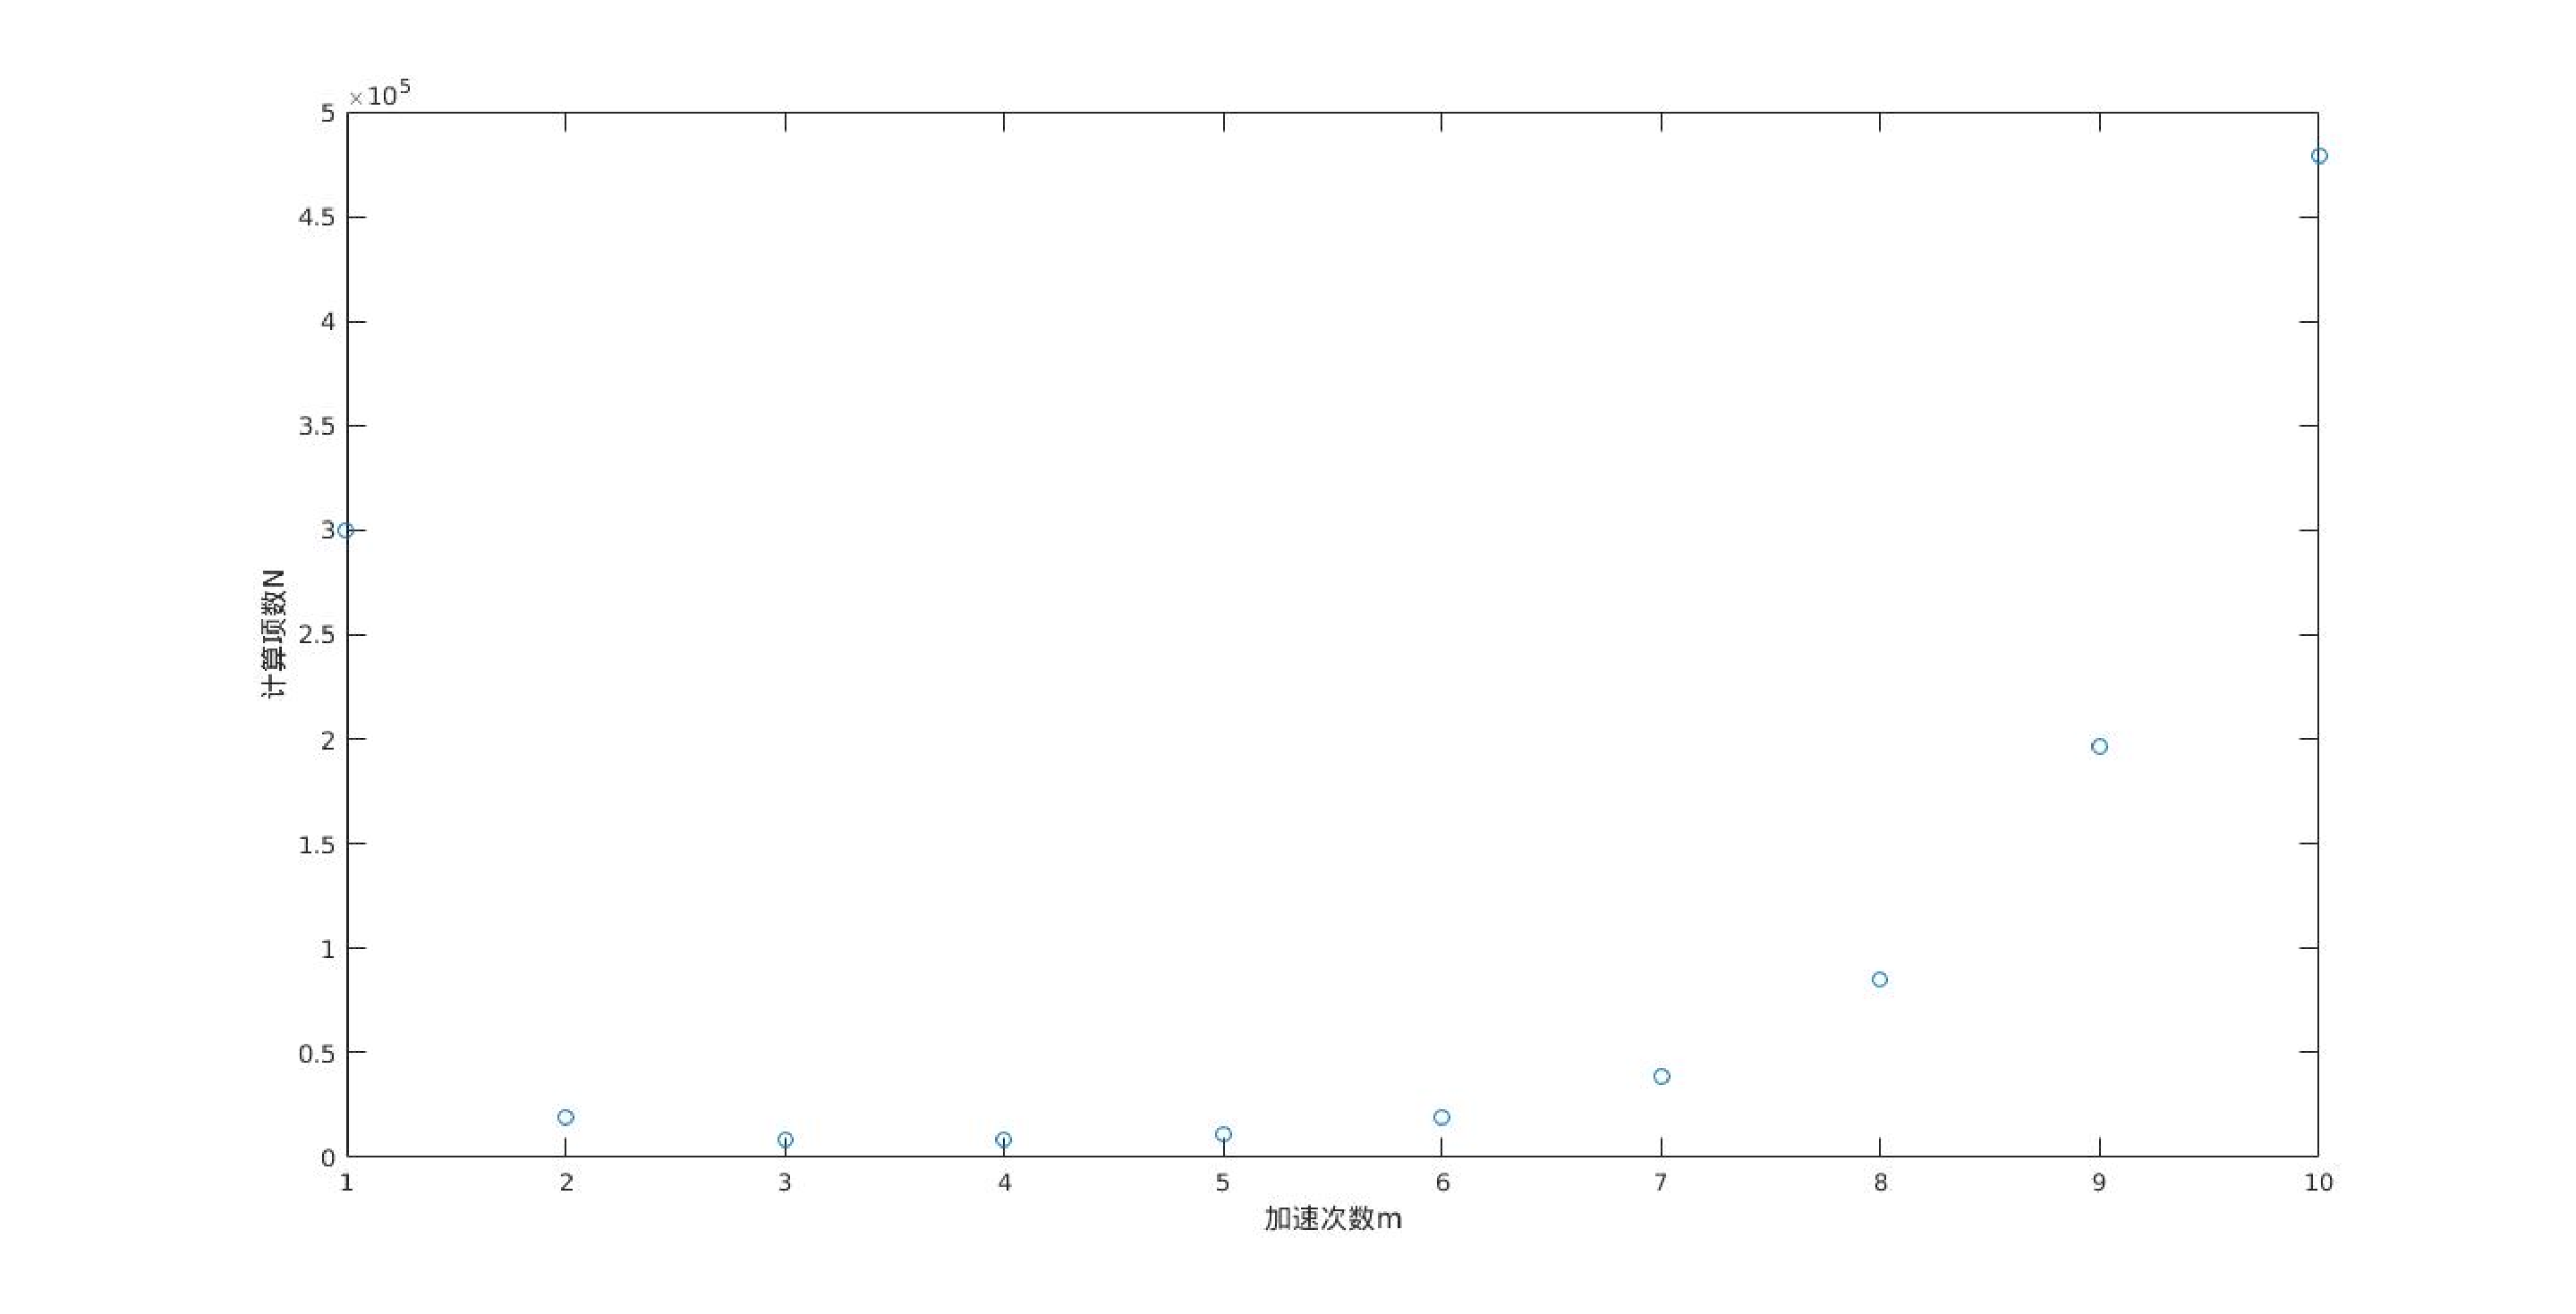
\includegraphics[width = .9\textwidth]{image/integration_m.eps}
\caption{加速次数与计算项数的关系}
\label{fig:integration_m}
\end{figure}
\subsection*{反双曲正切法}
通过查阅资料,发现了比泰勒级数更有效\cite{Logarithm_Wikipedia}的级数方法:基于反双曲正切的幂级数。
\begin{eqnarray*}
ln\left(t\right) &=&2*artanh\left(\frac{t-1}{t+1}\right)\\&=&2*\sum_{n=0}^{\infty}\frac{1}{2n+1}\left(\frac{t-1}{t+1}\right)^{2n+1}
\end{eqnarray*}

\section*{流程图}
\begin{figure}[H]
\centering
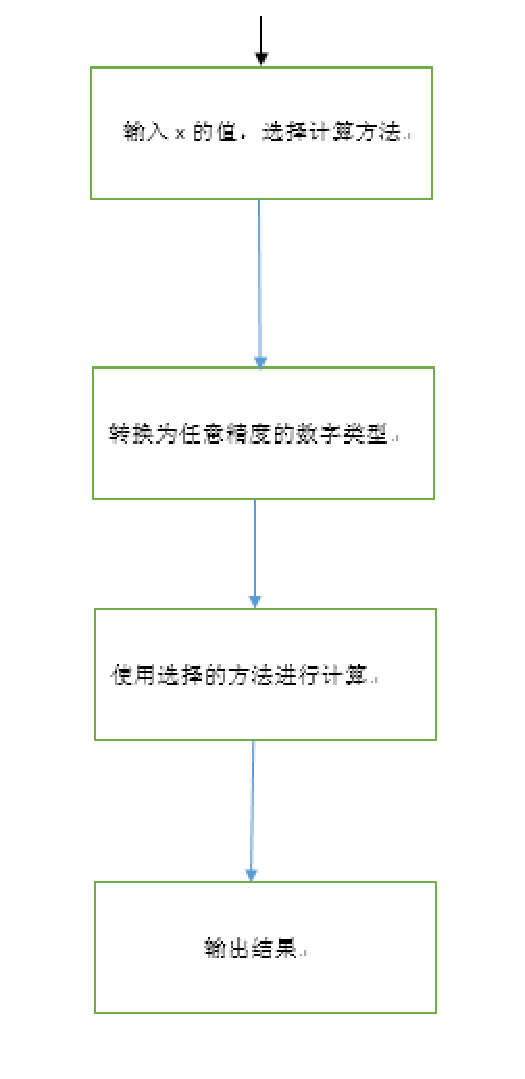
\includegraphics[width = .5\textwidth]{image/flowchart.eps}
\caption{流程图}
\label{fig:integration_m}
\end{figure}

\section*{误差估计}
\subsection*{泰勒级数法}
\subsubsection*{方法误差}
假设使用$N$项泰勒级数进行近似,则余项为级数$$R_N=\sum\limits_{n=N+1}^{\infty}\frac{\left(-1\right)^{n-1}*\left(t-1\right)^{n}}{n}$$
当$N$足够大时,此级数是绝对值单调下降的交错级数,即莱布尼茨级数。所以有结论$$\left|R_N\right| \le  \frac{\left(-1\right)^{N-1}*\left(t-1\right)^{N}}{N}$$对于输入$t\in\left(\frac{1}{e},1 \right]$有$$\left|R_N\right| \le \frac{\left(1-\frac{1}{e}\right)^N}{N}$$实验中取$N=100$所以有$$\left|R_N\right| \le 1.2*10^{-22}$$
\subsubsection*{存储误差}
\paragraph{}
实验中的中间各步计算都保持$25$位精度,$25$位之后的直接丢弃。乘法计算中先计算所有位数(即两个$25$位数相乘得到$50$位数),然后截取前$25$位。所以每一步加减法、乘除法的舍入误差都是$E=10^{-25}$。
\paragraph{}
因为$t\in\left(\frac{1}{e},1\right]$,所以$1-t < 1-\frac{1}{e}=\varepsilon$。考虑泰勒级数中每一项$a_k$的误差$e_k$有
\begin{eqnarray*}
&a_1=t-1 &e_1=E\\
&a_2=a_1*(t-1) &e_2=(1-t)E+e_1\\
&\cdot\cdot\cdot&\cdot\cdot\cdot\\
&a_k=a_{k-1}*(t-1) &e_k=(1-t)^{k-1}E+(1-t)e_{k-1} \le \varepsilon e_{k-1}+E\varepsilon^{k-1} \le \varepsilon e_{k-1}+E
\end{eqnarray*}
所以得到$$e_k \le \frac{1-\varepsilon^k}{1-\varepsilon}E \le \frac{E}{1-\varepsilon}$$所以存储误差$$R_2 \le \frac{E}{1-\varepsilon}*N=1.6*10^{-23}$$
\subsection*{数值积分法}
\subsubsection*{方法误差}
实验中使用的是龙贝格方法$R_N$,此方法的收敛速度为8阶。所以
\begin{eqnarray*}
R\left[f\right] &\le& h^8\\&=&\left(\frac{1-t}{N}\right)^8\\ &\le& \left(\frac{1-\frac{1}{e}}{N}\right)^8
\end{eqnarray*}
实验中取$N=300$,所以$$R \le 3.9*10^{-22}$$
\subsubsection*{存储误差}
因为每一项的误差上限是$E$,所以辛普生公式$S_n$的误差$R_{S_n}$满足$$R_{S_n} \le \frac{1}{6}\left(E+E+2(n-1)E+4nE\right) = nE$$由龙贝格公式与辛普生公式的关系得到$$R_{S_n} \le R_{S_{4n}}+R_{S_{2n}}+R_{S_{n}}=7NE=2.1*10^{-22}$$
\subsection*{反双曲正切法}
\subsubsection*{方法误差}
假设使用$N$项级数近似,则余项为$$\left|R_N\right| =  2*\sum_{n=N}^{\infty}\frac{1}{2n+1}\left(\frac{1-t}{t+1}\right)^{2n+1}$$所以
\begin{eqnarray*}
\left|R_N\right| &\le& 2*\sum_{n=N}^{\infty}\frac{1}{2N+1}\left(\frac{1-t}{t+1}\right)^{2n+1} \\ &=& \frac{2}{2N+1}\frac{\left(\frac{1-t}{t+1}\right)^{2N+1}}{1-\left(\frac{1-t}{t+1}\right)^2}\\&\le& \frac{2}{2N+1}\cdot\frac{\left(\frac{1-\frac{1}{e}}{\frac{1}{e}+1}\right)^{2N+1}}{1-\left(\frac{1-\frac{1}{e}}{\frac{1}{e}+1}\right)^2}\\&=&\frac{2}{2N+1}\cdot\frac{\left(0.462\right)^{2N+1}}{0.786}
\end{eqnarray*}
实验中取$N=30$,所以$$\left|R_N\right| \le 1.5*10^{-22}$$
\subsubsection*{存储误差}
因为$t\in\left(\frac{1}{e},1\right]$,所以$\left(\frac{1-t}{1+t}\right)^2 \le \left(\frac{1-\frac{1}{e}}{\frac{1}{e}+1}\right)^2=\varepsilon$。考虑级数中每一项$a_k$的误差$e_k$有
\begin{eqnarray*}
&a_1=\frac{1-t}{1+t} &e_1=E\\
&a_2=a_1*\left(\frac{1-\frac{1}{e}}{\frac{1}{e}+1}\right)^2 &e_2=\left(\frac{1-\frac{1}{e}}{\frac{1}{e}+1}\right)^3E+e_1\\
&\cdot\cdot\cdot&\cdot\cdot\cdot\\
&a_k=a_{k-1}*\left(\frac{1-\frac{1}{e}}{\frac{1}{e}+1}\right)^2 &e_k=\left(\frac{1-\frac{1}{e}}{\frac{1}{e}+1}\right)^{2k-1}E+\left(\frac{1-\frac{1}{e}}{\frac{1}{e}+1}\right)^2e_{k-1} \le \varepsilon e_{k-1}+E\varepsilon^{k-1} \le \varepsilon e_{k-1}+E
\end{eqnarray*}
所以得到$$e_k \le \frac{1-\varepsilon^k}{1-\varepsilon}E \le \frac{E}{1-\varepsilon}$$所以存储误差$$R_2 \le \frac{E}{1-\varepsilon}*N=6.4*10^{-24}$$
\section*{结果分析}
\subsection*{收敛速度}
\paragraph{两种幂级数方法进行比较}
在同等精度下,反双曲正切级数比泰勒级数用的项更少。假设后者使用$N$项,则前者使用小于$\frac{N}{2}$项即可,收敛更快。
\paragraph{幂级数法与龙贝格积分法进行比较}
龙贝格方法需要更多的计算,才能达到相同精度
\subsection*{计算时间}
进过测试,泰勒级数和反双曲正切级数法的用时都小于$0.1s$,而积分法则需要$3s$左右的时间
\subsection*{数据测试}
使用$1,2,3,\cdot\cdot\cdot,100$进行了测试,三种方法计算结果前$21$位完全一致
\newpage
%如果文档类是article之类的, 用\renewcommand\refname{参考文献}
\renewcommand\refname{参考文献}
\bibliographystyle{plain}
\bibliography{ref.bib}
\end{document}
